Following the calibration of the Agent-Based Model (ABM), the study encountered significant computational and behavioral challenges during the initial training phase of the Deep Reinforcement Learning (DRL) agent. These challenges necessitated critical architectural deviations from the initial thesis proposal, specifically regarding the reinforcement learning framework, the reward optimization algorithm, and the mathematical stability of the household agents. This section details the quantitative results that justified the transition to the Heuristic-Guided (HuDRL) framework and the integration of a ``Social Norm Shield'' to prevent unrealistic compliance volatility.

\subsection{Overcoming the Sparse Reward Problem via Action Masking}
Even with an interactive environment, a fundamental challenge emerged: the \textit{Sparse Reward Problem} inherent to the high-dimensional continuous action space ($d=21$). The initial assumption was that a standard Proximal Policy Optimization (PPO) agent could autonomously discover the optimal ``Sequential Saturation'' strategy given sufficient training episodes. 

In the baseline non-heuristic implementation, the unguided neural network was required to simultaneously optimize continuous budget allocations across three distinct policy levers for seven heterogeneous barangays. The probability of the agent randomly initializing a policy that concentrated massive resources on a single struggling barangay was mathematically negligible. Instead, the baseline PPO agent rapidly converged to a local optimum characterized by "safety-seeking" behavior. It learned to distribute funds equally across the grid to minimize the risk of triggering the Political Collapse penalty, resulting in heavily diluted interventions that completely failed to overcome the citizens' behavioral inertia \citep{ZhengAI2022}. 

To resolve this, the methodology transitioned to the Heuristic-Guided (HuDRL) framework. As detailed in the system architecture, this involved introducing a Temperature-Scaled Softmax function ($\tau=5.0$) to violently amplify the AI's highest confidences, forcing polarized budget concentrations. Furthermore, a Safety-Critical Action Mask was integrated—specifically the 70\% Graduation Rule and the 50\% Phase-Shift Crisis Guardrail—which programmatically blocked the AI from wasting funds on stable areas or starving critical sectors during its random exploration phase.

\subsection{Comparative Convergence: Heuristic vs. Non-Heuristic PPO}
To evaluate the efficacy of these methodological refinements, the simulation benchmarked the HuDRL architecture against the baseline Non-Heuristic PPO approach over a 12-quarter horizon. Figure \ref{fig:heuristic_vs_non_heuristic} illustrates the Global Compliance Rate trajectories for both models relative to the defined Stability Threshold ($70\%$) and Collapse Zone ($<40\%$).

\begin{figure}[htbp]
    \centering
    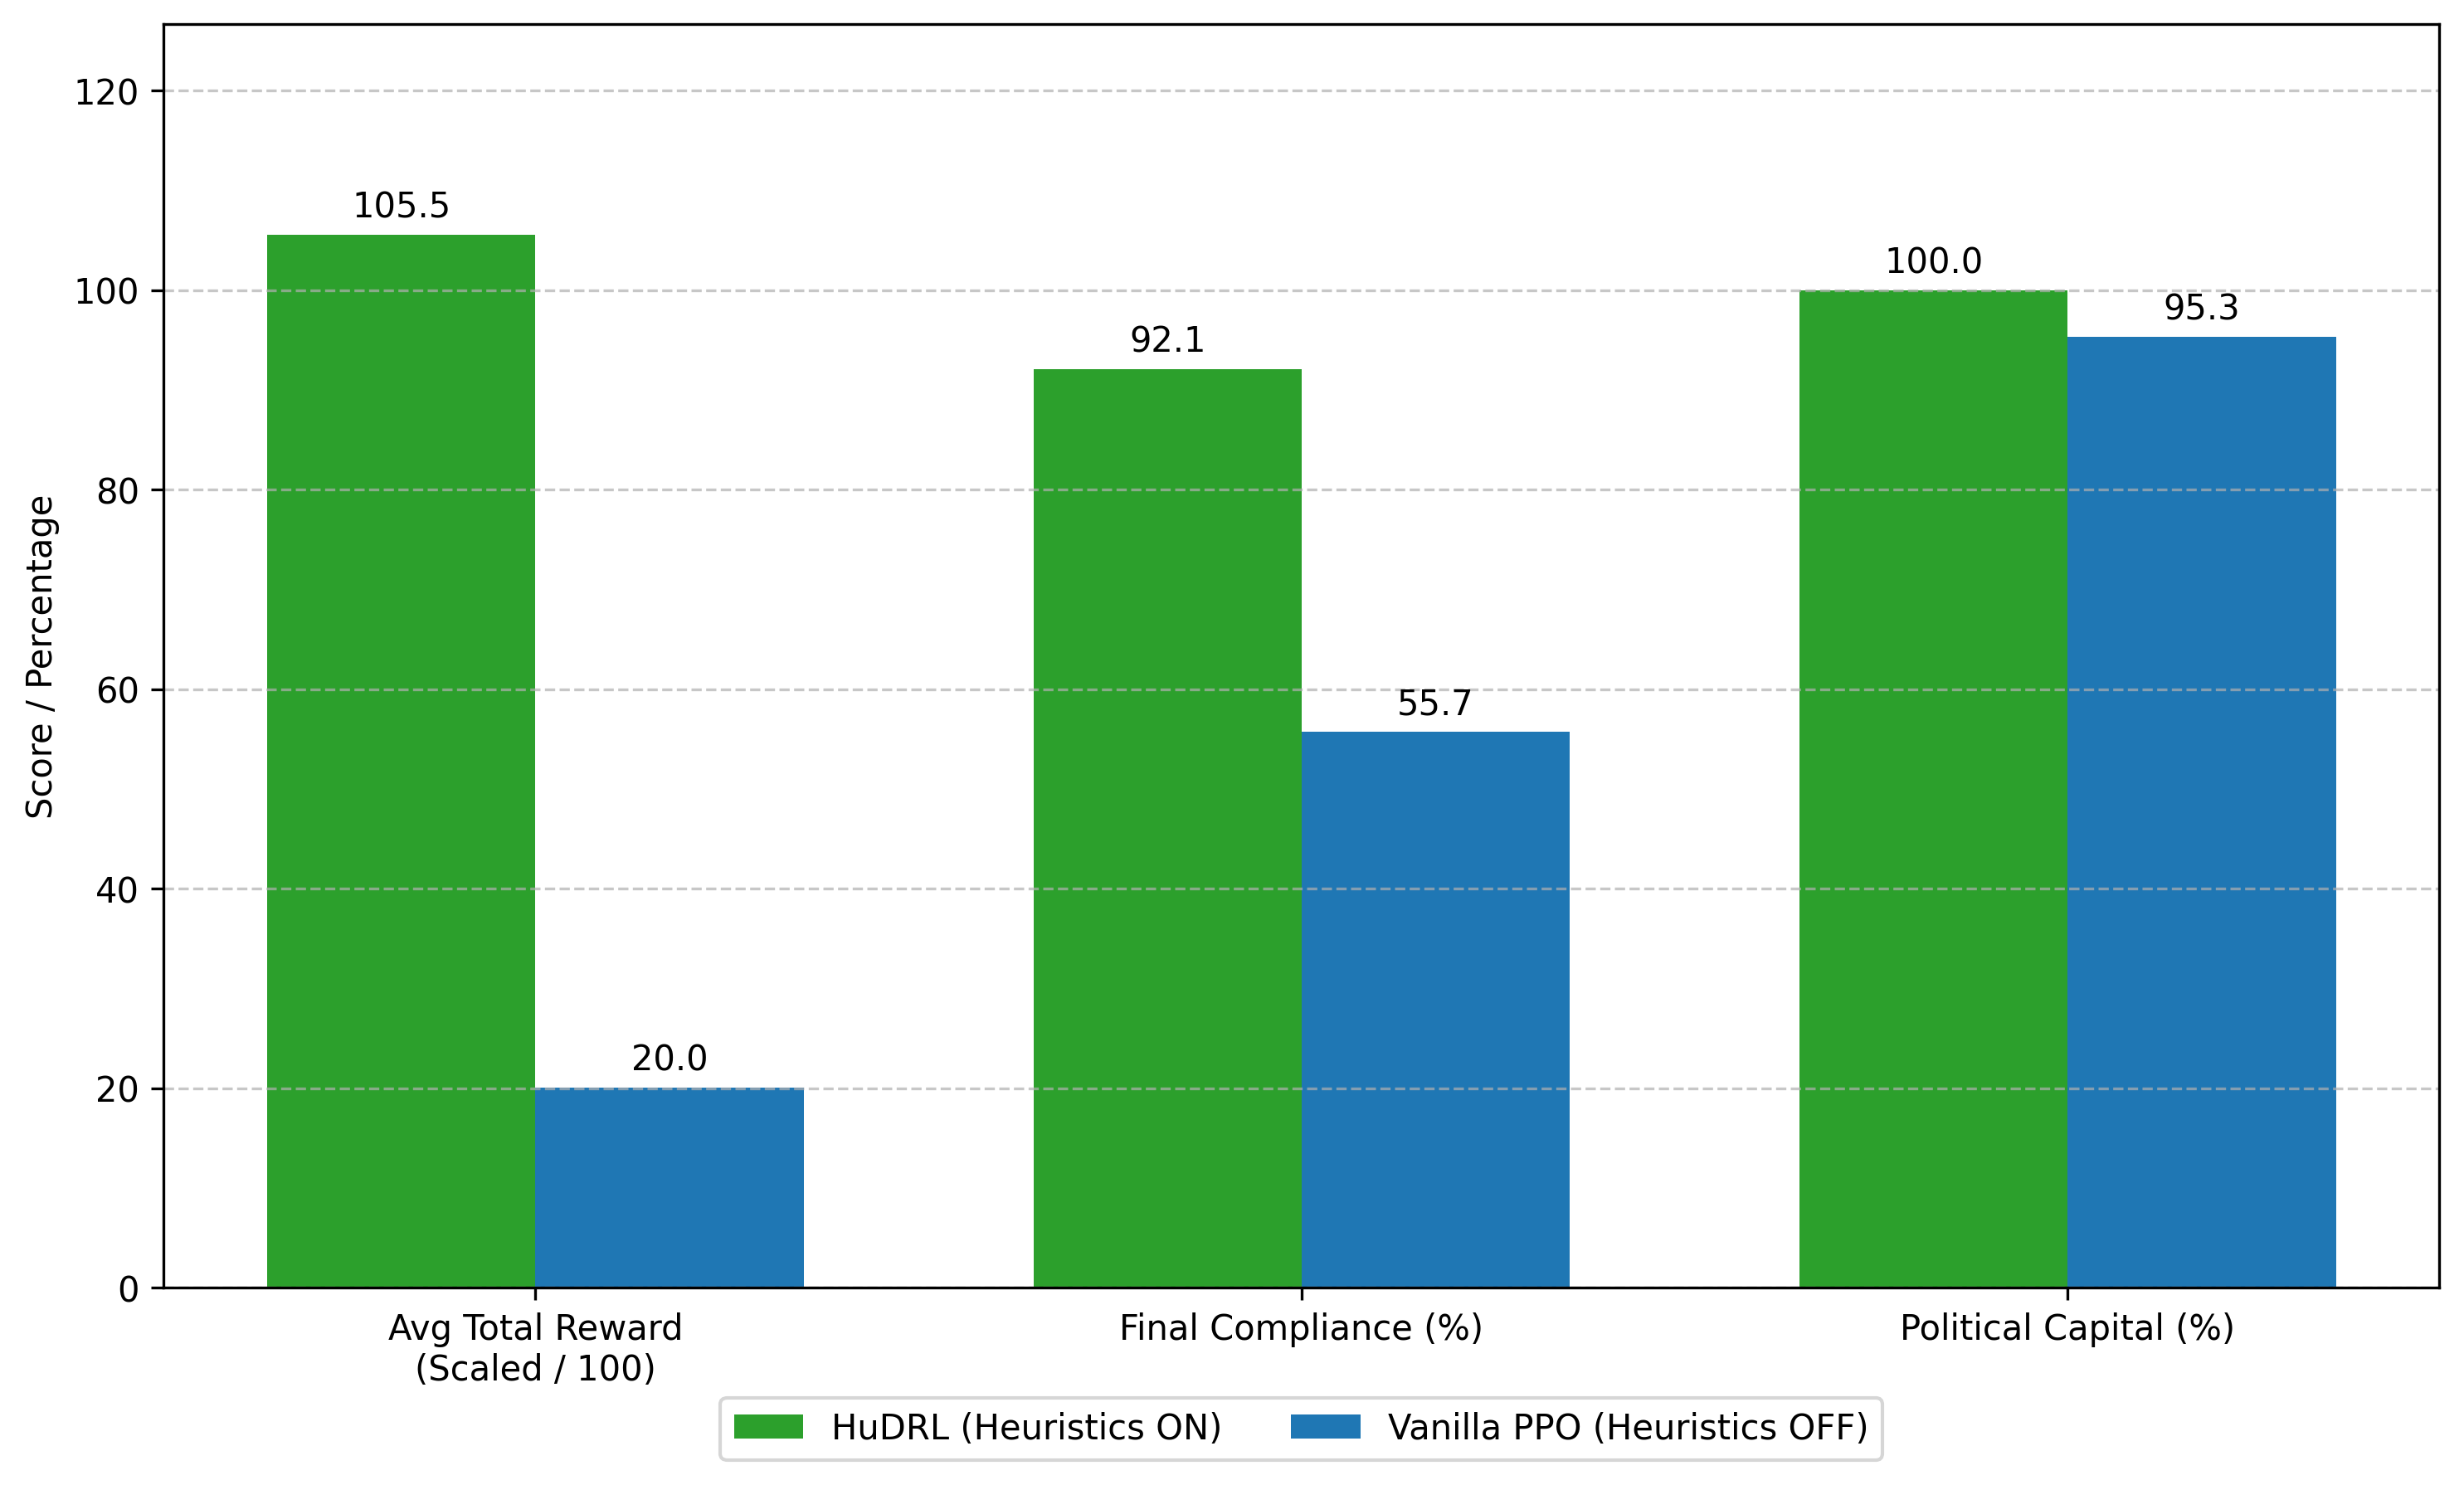
\includegraphics[width=0.9\textwidth]{images/hudrl_vs_vanilla.png}
    \caption{Categorization of Systemic Compliance Zones and Stability Thresholds}
    \label{fig:heuristic_vs_non_heuristic}
\end{figure}

The \textbf{Non-Heuristic Approach} (represented by the dashed grey trajectory) exhibited severe policy stagnation. Throughout the entire 3-year simulation timeline, the global compliance rate remained virtually flat at approximately $20\%$. This performance consistently trapped the municipality within the ``Collapse Zone,'' mathematically proving that without heuristic action-masking or adaptive triage logic, the system failed to concentrate enough capital to incentivize behavioral change.

In stark contrast, the \textbf{Heuristic Approach} (solid blue trajectory) demonstrated rapid gradient convergence toward optimal compliance. Starting at a baseline compliance rate of $51.8\%$ in Quarter 1 (under the guided framework), the HuDRL agent successfully navigated the non-convex policy space, breaching the critical $70\%$ Stability Threshold by Quarter 2. By systematically targeting failing sectors via the algorithmic guardrails, the system achieved a near-saturation point by Quarter 6, reaching approximately $98\%$ compliance, and maintained this asymptotic stability through Quarter 12. 

\subsection{Heuristic Reward Design and Population Density Bias}
During the refinement of the HuDRL reward structure, a critical design choice involved defining the optimal heuristic rule to guide the agent's spatial targeting. The study conducted trial benchmarks comparing two distinct reward formulations:
\begin{enumerate}
    \item \textbf{Algorithm 1 (Maximin Triage):} Penalized the agent purely based on the barangay with the lowest absolute percentage of compliance, completely blinding the AI to the local household population size.
    \item \textbf{Algorithm 2 (Density-Weighted):} Factored in both low compliance and high household population density, operating on the theoretical assumption that targeting densely populated urban centers would maximize the raw number of compliant households per budget cycle.
\end{enumerate}

Empirical testing revealed a severe algorithmic flaw in Algorithm 2, rooted in "population density bias" \citep{Mehrabi2021}. Because the PPO objective function seeks to maximize cumulative scalar rewards, the agent discovered a mathematical exploit. It developed a learned propensity to disproportionately funnel funds into the massive urban center (Barangay Poblacion, $N=1,534$), even when its compliance was only marginally below optimal levels. For the AI, shifting a massive population by merely 2\% yielded a higher absolute numerical reward than fully stabilizing a sparsely populated rural barangay (e.g., Babalaya, $N=171$) failing at 10\% compliance.

This generated severe systemic inequality. The agent continuously harvested "cheap" marginal rewards from high-density areas, abandoning rural nodes in the Collapse Zone indefinitely. This computational behavior perfectly mirrors algorithmic public policy failures, where optimizing strictly for aggregate efficiency reinforces systemic inequities against low-density populations \citep{Alphonso2024}. To resolve this reward exploitation, the final HuDRL framework adopted Algorithm 1. By blinding the agent to density, the heuristic enforces the \textit{Maximin} equity principle (maximizing the minimum), compelling the AI to execute systematic "bottleneck resolution" \citep{TianReview2024}.

\subsection{Addressing Behavioral Volatility via the Social Norm Shield}
The final major algorithmic refinement addressed the behavioral stability of the \texttt{HouseholdAgents}. Early headless simulations exhibited a phenomenon of ``Instantaneous Collapse,'' where compliance rates in a stabilized barangay would plummet from 90\% to near 0\% in a single quarter the moment the Mayor Agent withdrew its strike force or incentive budget.

While mathematically faithful to the raw Theory of Planned Behavior (TPB) decay equations, this volatility was sociologically unrealistic. Real-world populations exhibit cultural hysteresis, where established habits persist long after the removal of external financial stimuli \citep{Nishimura2022}. To correct this computational artifact, the study implemented a ``Social Norm Shield,'' governed by two empirically tuned thresholds:

\begin{itemize}
    \item \textbf{The Tipping Point (70\%) and Deterministic Lock:} The model assumes that once a localized node breaches 70\% compliance, the behavior transitions from ``incentive-driven'' to ``norm-driven.'' Consequently, the simulation executes a deterministic hard-lock on the Subjective Norm ($w_{sn}$) variable, preventing standard dynamic decay. This simulates the non-linear phase transitions characteristic of collective behavior models \citep{Centola2018}. Implementing a continuous decay curve would falsely imply that social conventions instantly erode without constant government funding, contradicting the ``ratchet effect'' observed in environmental sociology \citep{Andre2021, Nyborg2024}.
    
    \item \textbf{The Social Norm Floor (40\%):} To prevent total mathematical collapse during the DRL agent's early exploration phase, an absolute floor was implemented. Even under zero enforcement, spatial peer pressure prevents compliance from dropping below 40\%. This bounds the agents' baseline behavior, simulating the internalized ``moral obligation'' and residual cultural memory identified in regional waste management studies \citep{Zheng2022}.
\end{itemize}

This refinement was mathematically paramount. By enabling cultural hysteresis, the HuDRL agent could successfully execute its ``Sequential Saturation'' strategy—concentrating municipal capital to conquer one barangay, locking in its social norms, and safely relocating its budget to the next target without the first node immediately collapsing behind it \citep{Abdallah2021}.